\section{Methodology}
\subsection{Historical evidence and data provenance}
Table~\ref{tab:master} summarizes the executed design. The preserved historical study contains 8005 shared time rows, CPU and memory, 28 services, a 12-step input and one-step (30-minute) forecast. It uses three training seeds, twenty mask realizations and seven conditions: complete telemetry and scattered/short-block losses at 10\%, 20\% and 40\%. Its E0--E5, C0--C3, V2 and original comparators remain available. V2 selects an already trained compact family using source validation; it is not an additional independently trained model. A historical prediction-manifest audit checks the preserved files. Their errors must not be combined with new-service errors as if the two cohorts were independent replications.

ChronoGraph provides nominally half-hour samples. The publisher describes 708 services and 1529 edges in the full graph \cite{chronograph}. The analyzed cohorts are induced subsets, with no use of all 708 services for model fitting. We retain chronological row cuts $[0,5603)$, $[5603,6404)$ and $[6404,8005)$, giving 70/10/20 proportions to rounding. These proportions refer to rows, not elapsed wall time: one 108000-second jump occurs after row 5907 in validation. Windows and MASE consecutive pairs do not cross that gap. The source cohort is unchanged. Its induced subgraph retains 28 internal edges and excludes 137 boundary edges. A separate 32-service cohort is chosen using static topology and a reproducible SHA-ranked traversal, excluding the original 28 services and four known pilot services. Selection does not use forecast errors. This connected convenience cohort is not a random sample of microservice populations.

All weights and hyperparameters use source training/validation only. For each destination service, mean, standard deviation, median and the MASE denominator use its first 5603 rows. Destination validation rows do not select models. This is \emph{calibrated spatial transfer}: it is not strict zero-shot forecasting without destination data. CPU stays on the publisher's scale; memory is in bytes. No conversion to CPU cores or percentage is assumed. The static destination graph supplies new adjacency buffers for graph models, with no new learned weights. Its edge-availability dates are not fully established.

The external case uses the first 48 official Alibaba 2022 \texttt{MSMetricsUpdate} objects, covering one day \cite{alibaba2022}. The source archive totals 17,890,753,336 bytes and 675,424,445 pod CSV rows. A bounded download queue checks the owner's Content-MD5 values and records SHA-256 values. Thirty-two service names are chosen by a SHA ranking among services covering every timestamp in the initial object; they are then placed in lexicographic order. Selection uses availability rather than forecast performance. For each timestamp, pod values with both resource fields finite are averaged by service. Those timestamp means receive equal weight in a completed half-hour bin. Bins with fewer than 30 valid minute observations are missing. Their means become available only at bin close, so no future bin values enter an input.

Alibaba's published resource values are min--max normalized utilization, not physical cores or bytes. The temporal scope of the provider's normalization is undocumented here. The processed case has 48 bins; the first 12 bins (six hours) supply calibration statistics and may appear in past input windows. The remaining 36 bins are forecast targets. Four scalar values are naturally missing in calibration only, corresponding to two service/bin pairs in both resources; no evaluation target is imputed. Frozen L12, one-step source weights are transferred without external fitting or tuning. GRU with graph is excluded because the external call graph was not acquired. This external design is deliberately distinct from the 70/10/20 source experiment and supplies only a short, exploratory cross-dataset case.

\subsection{Causal preparation and synthetic missingness}
Let $y_{t,s,r}$ be the recorded target at time $t$, service $s$ and resource $r$. Each resource is forecast separately. The input contains $L$ prepared steps ending at $t-h$, and the direct scalar output predicts $y_{t,s,r}$. Partition boundaries and temporal gaps reset the preparation. Normalization uses the corresponding training-prefix statistics; the standard deviation has a numerical floor of $10^{-8}$. Calibration statistics precede synthetic masking. The study therefore does not test learning those statistics from synthetically degraded calibration data.

At each step, an observed value is retained, a missing value uses the last available observation, and the training median is used until the first observation in the segment. Define $m$ as the observation indicator, $c$ as missing-after-an-observation and $f$ as missing-before-any-observation; $m+c+f=1$. The age $\delta$ counts missing steps since the latest available sample. Prepared channels contain the filled normalized value, $m$, $\log(1+\delta)/\log(1+L)$, $c$ and $f$. Inputs contain no target-time information. However, the propagated value and its age can summarize an observation older than the nominal $L$-step window; $L$ is not a strict upper bound on historical information.

Seven original conditions are retained. Scattered losses select an exact rounded number of unavailable entries per service/segment. Short-block losses allocate that count using candidate blocks of at most six steps. Three additional conditions use nominal 20\% loss: correlated masks shared within consecutive lexicographic groups of eight services; prolonged candidate blocks of at most 24 steps; and lag-dependent MAR. The block construction leaves separators and can truncate the final selected block to meet the exact count. These are simulated monitoring mechanisms, not recorded outages.

The lag-MAR probability at a step is
\begin{equation}
 p_t=0.2\{1+0.5\tanh(|z^{\mathrm{last,CPU}}_t|)\},
\end{equation}
where $z^{\mathrm{last,CPU}}_t$ is based on the latest \emph{previously observed} normalized CPU. Thus $0.2\leq p_t<0.3$; ``20\%'' is a nominal condition label, not its realized rate. A shared induced mask applies to both resources, intersected with their natural availability. Twenty paired mask seeds are used in the primary setting, identically across model families and training seeds. Their sequence was already used historically; new-service evaluation does not make that sequence unseen. Fig.~\ref{fig:masks} displays actual generated masks. Fig.~\ref{fig:temporal} illustrates the cut positions and forecast origin.

\begin{figure*}[t]\centering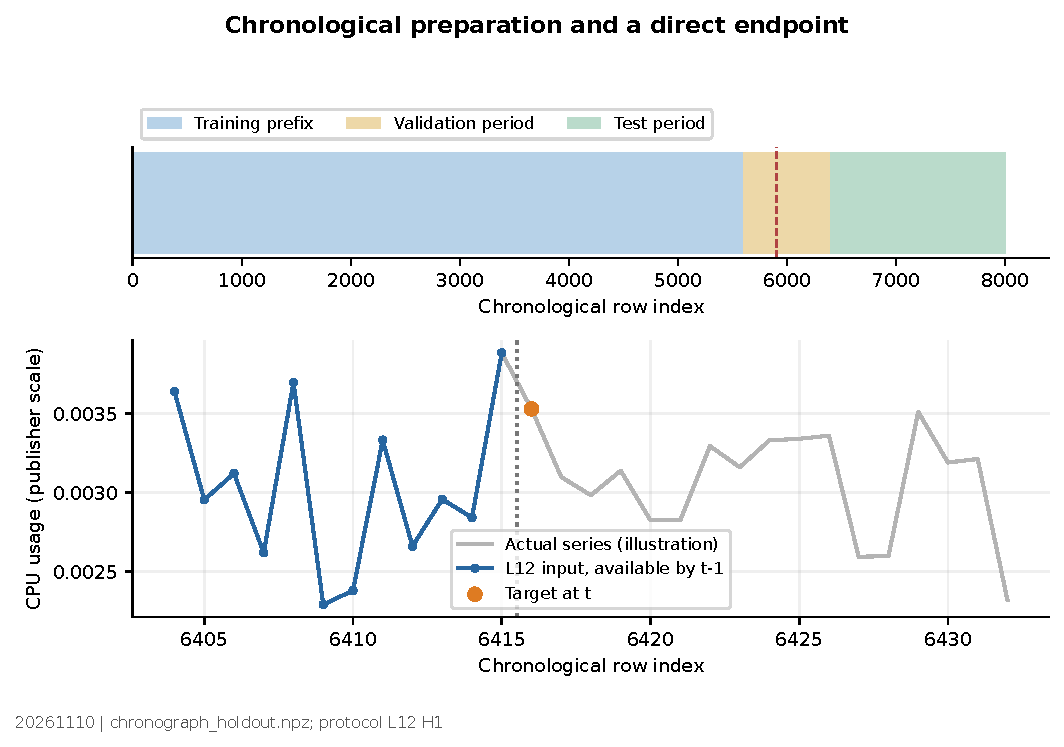
\includegraphics[width=0.72\textwidth]{figuras/04_temporal_preparation.pdf}
\caption{Row-based chronological preparation. The gap after row 5907 belongs to validation. The lower panel uses actual service values to illustrate an L12/H1 input; grey later values are displayed for context and are excluded from the forecast input.}\label{fig:temporal}\end{figure*}

\begin{figure*}[t]\centering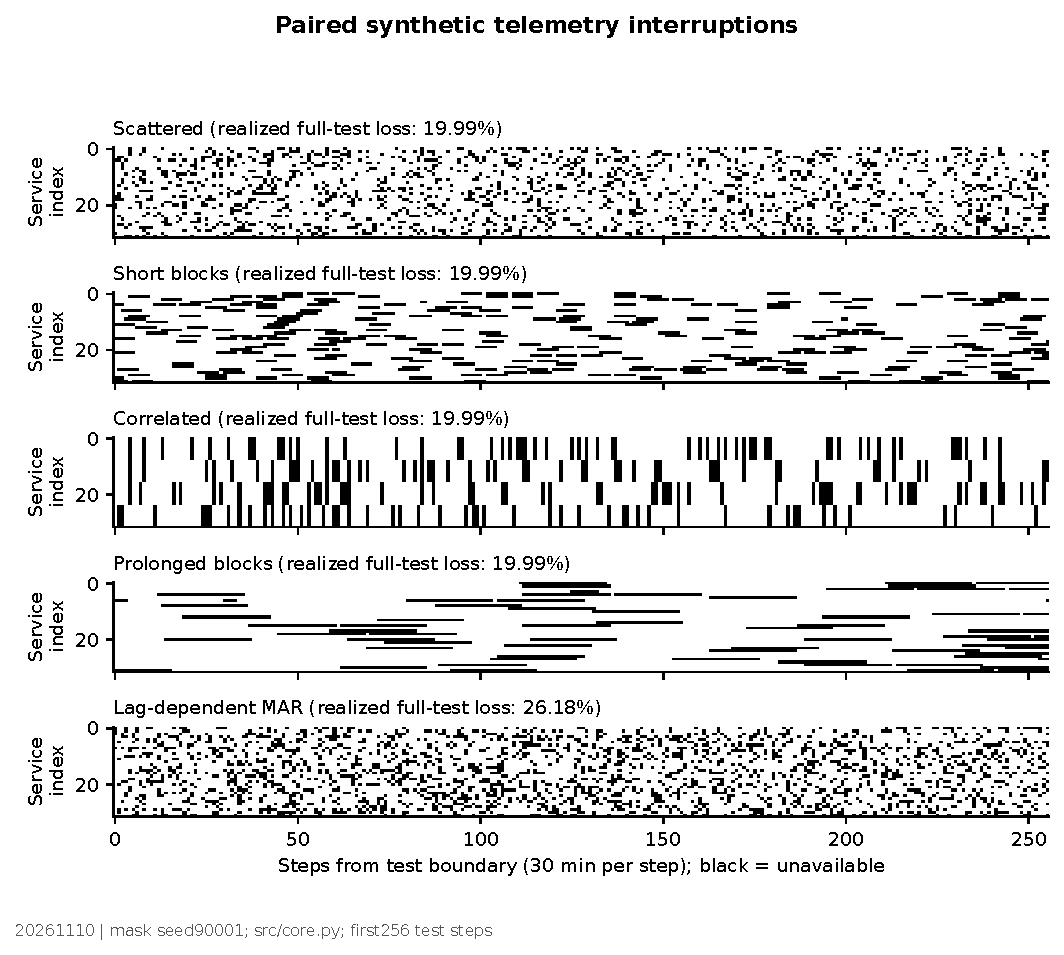
\includegraphics[width=0.68\textwidth]{figuras/05_missingness.pdf}
\caption{Actual masks generated from seed 90001, showing the first 256 test steps. Black indicates unavailability. Correlated groups and block duration are imposed mechanisms. Lag-MAR's probability varies and is not an exact 20\% loss condition.}\label{fig:masks}\end{figure*}

\subsection{Fixed decomposition and compact availability descriptors}
For a filled window $v\in\mathbb{R}^{L}$ and a fixed linear smoothing matrix $S$, DLinear is
\begin{align}
 \widehat x&=w_t^\top Sv+w_r^\top(I-S)v+b_t+b_r\nonumber\\
 &=\underbrace{[S^\top w_t+(I-S)^\top w_r]}_{w_{\rm eff}}^\top v+\underbrace{b_t+b_r}_{b_{\rm eff}}.
\end{align}
The implementation uses a fixed MA25 with replicated padding, including when $L=12$. The centered filter uses only the already available input window; it does not access future forecast targets. Its residual is not established to be a seasonal component. The two-head and collapsed forms define the same affine function class, but Adam and weight decay need not follow equivalent trajectories in the two parameterizations.

A0 uses $w_{\rm eff},b_{\rm eff}$ as a single affine head. A1 adds the window missing fraction $u=L^{-1}\sum_i(1-m_i)$; A2 adds the final log-age $a=\log(1+\delta_{\rm last})/\log(1+L)$; and A3 adds both:
\begin{equation}
 \widehat x_{\mathrm{A3}}=w^\top v+b+\gamma u+\eta a.
\end{equation}
The A0--A3 value function is initialized from the same seeded DLinear heads; additional coefficients start at zero. Float32 initialization equivalence is checked with relative tolerance $10^{-5}$ and absolute tolerance $10^{-6}$, not bitwise equality. The log-age is not clipped in A2/A3. Their parameter counts are $L+1,L+2,L+2,L+3$, versus $2L+2$ for DLinear. The proposal is a parameterization and descriptor study, not a new linear function class. Each family is independently tuned, so these comparisons do not isolate descriptor effects at identical selected hyperparameters.

E5 preserves the historically chosen availability-dependent EMA coefficient $\alpha=0.7$, observation, carry and fallback descriptors and a linearly capped age channel. It has $6L+2$ parameters. Its mask-dependent decomposition is not the fixed $S$ used in the algebraic collapse above. A3 is therefore not an exact collapse of E5. Figs.~\ref{fig:dlinear} and~\ref{fig:a3} show these model distinctions.

\begin{figure*}[!t]\centering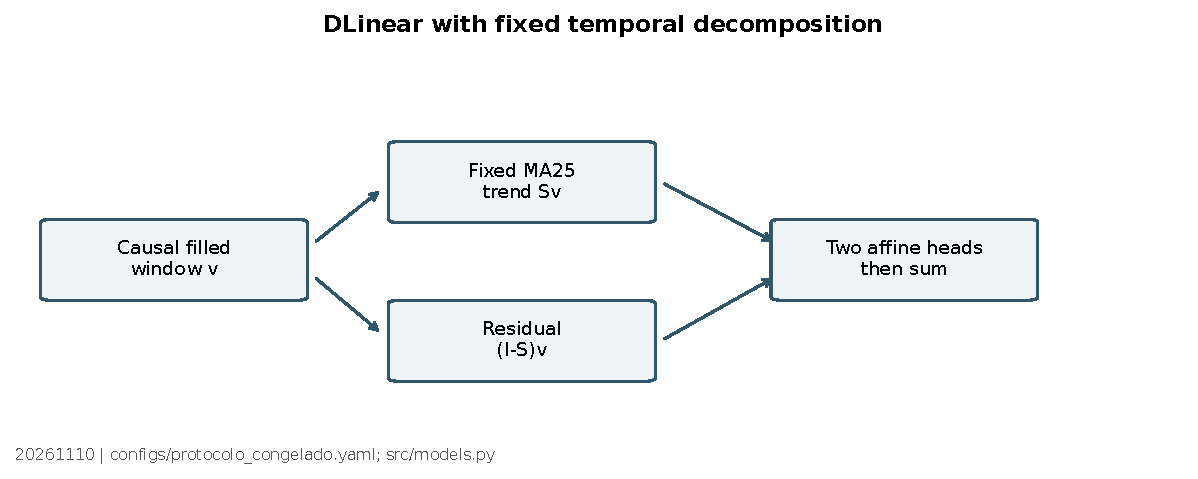
\includegraphics[width=0.79\textwidth]{figuras/02_dlinear.pdf}
\caption{Fixed DLinear decomposition. Both filtered components depend only on the available past window. A fixed smoothing matrix permits algebraic collapse to an affine head, without guaranteeing an identical optimizer trajectory.}\label{fig:dlinear}\end{figure*}

\begin{figure*}[!t]\centering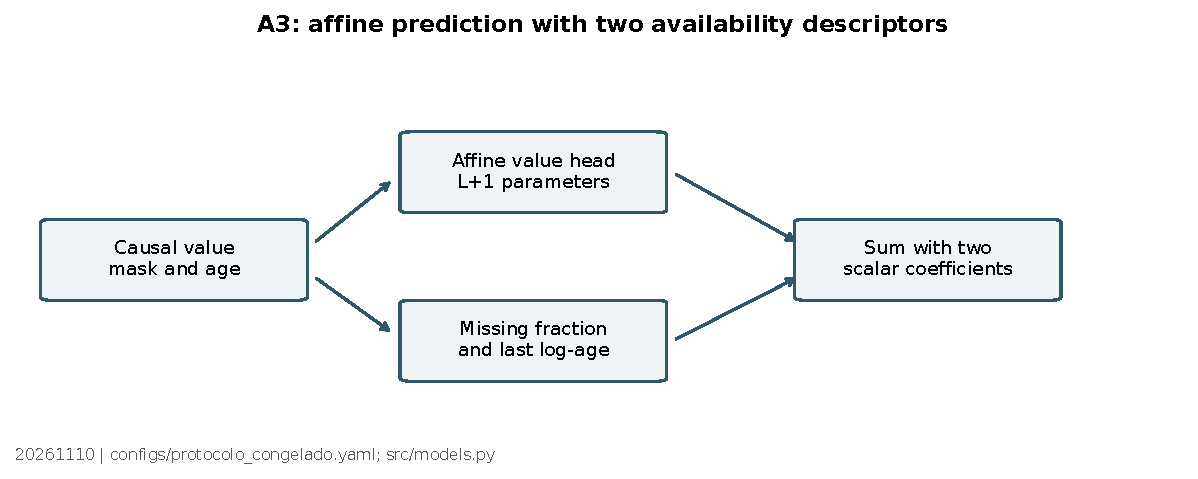
\includegraphics[width=0.79\textwidth]{figuras/03_a3.pdf}
\caption{A3 adds missing fraction and last log-age to the collapsed affine value head. With L12 it uses 15 trainable parameters per resource. Extra coefficients start at zero; descriptor families are tuned independently.}\label{fig:a3}\end{figure*}

\subsection{Historical decomposition, compact families and selection}
The original E0 is fixed MA25 DLinear with 26 trainable parameters per resource. E1 selects a moving-average width from 3, 7, 13 and 25. E2 replaces its level with an observation-updated exponential component. For prepared value $v_i$, indicator $m_i$ and initial level $\ell_1=v_1$, the recurrence is
\begin{equation}
\ell_i=\ell_{i-1}+\alpha m_i(v_i-\ell_{i-1}),\qquad r_i=v_i-\ell_i.
\end{equation}
The historical search considered fixed $\alpha=0.1,0.3,0.7$ and a sigmoid-constrained learned scalar; the selected final configurations use fixed factors. E3 adds a bias-free projection of the 36 availability/carry/fallback indicators, E4 adds a bias-free projection of twelve ages, and E5 combines the exponential component with both heads. Thus E3, E4 and fixed-factor E5 contain 62, 38 and 74 parameters. The added heads start at zero. Because the three status indicators sum to one and positive age also reveals absence, the ablations do not identify orthogonal causal information effects.

The C families retain the two-head decomposition. They add at most a missing-fraction coefficient and a final-age coefficient:
\begin{equation}
\widehat x_C=\widehat x_{\rm base}+\gamma_p L^{-1}\sum_i(1-m_i)+\gamma_a a_L.
\end{equation}
C0 includes neither coefficient, C1 only missing fraction, C2 only age, and C3 both; parameter counts are 26, 27, 27 and 28. Each selects among MA25, EMA0.3 and EMA0.7. These families differ from A0--A3: the A families collapse the fixed DLinear value heads and contain 13--15 parameters at L12, whereas the C families preserve 26 base parameters. Fig.~\ref{fig:evolution} summarizes this progression. A3 is neither the validation alias V2 nor a simple relabeling of C3.

Historical training uses Adam, learning-rate candidates 0.001/0.003, normalized MSE, gradient clipping at one, batch16, up to twenty epochs and patience five. A rotating condition assignment is modulo seven. The short historical search uses three epochs, 512 training origins and 32 validation origins, with selection details that differ across the original variants. C0--C3 use a common six-candidate decomposition/rate grid per resource: 48 short fits followed by 24 final fits across both resources and three seeds. V2 selects one family per resource using the mean best validation MASE of the three seeded fits, breaking ties by parameter count and family identifier. It reuses that family's weights and predictions. No service-specific or test-time oracle selects V2 outputs.

For L12/H1, the historical valid-origin counts are 5591 training, 777 validation and 1589 test. Origin eligibility respects both the row partitions and the actual time gap. Twenty paired realizations cover seven original conditions. Historical uncertainty uses 10000 resamples of whole mask realizations, seed91001, and a crossed three-seed/twenty-mask sensitivity. The historical percentage reduction is calculated after averaging within each mask realization. The expanded percentage estimand instead averages paired service-level cell percentages. These definitions are retained rather than equated merely because both are called reductions.


\subsection{Comparator implementations}
The simple references are persistence, moving average, exponential smoothing and ridge regression with an intercept. Moving-average candidates are 1, 3, 6 and 12 steps, even for longer input windows. Exponential smoothing uses $\alpha\in\{0.1,0.3,0.7,0.9\}$ and updates only on available measurements. Ridge uses $\lambda\in\{0,10^{-4},10^{-2},1\}$, with the intercept unpenalized, fitting all ten prepared training conditions analytically. DLinear, NLinear and the A/E families share their weights across services and predict one resource at a time.

The GRU variants use hidden width 12 and nine input channels per step. GRU (own) repeats the local value/mask/age triplet in three slots to match the graph model's input width. GRU (graph) replaces two slots with incoming and outgoing row-normalized graph aggregates; it contains 841 trainable parameters, as does the width-matched local comparator. The GRU-D adaptation has 615 parameters, decays the input toward normalized mean zero, decays its hidden state and uses a GRU cell with value/mask inputs. This shared-service adaptation is not the canonical clinical multivariate experiment.

PatchTST uses the official Apache-2.0 code at commit \texttt{204c21efe0b3} (full identifier in the code manifest): one input channel, patch length 4, stride 2, end padding, one layer, model width 16, two heads, feed-forward width 32, dropout 0.1 and affine RevIN. The output is the single direct endpoint. At L12 it has 2499 trainable elements plus one fixed attention-scale element registered as a non-trainable parameter. Frozen checkpoint metadata counting all parameter tensors is preserved, while reported trainable counts filter \texttt{requires\_grad}. Calibration, graph buffers, optimizer states and input caches are outside the trainable-count definition. This compact recipe does not reproduce PatchTST's published benchmark settings. TimesNet, iTransformer, TimeMixer and TiDE are not executed in the new queue; historical BiTGraph and GinAR results remain visible separately.

\subsection{Prediction maps and recurrent inputs}
For prepared history $v$, the persistence prediction is $v_L$. Moving average uses $k^{-1}\sum_{i=L-k+1}^L v_i$, and simple exponential smoothing uses the last state of the availability-updated recurrence above. Ridge minimizes $\sum_j(x_j-w^\top v_j-b)^2+\lambda\|w\|_2^2$ over prepared source examples $j$. NLinear predicts $v_L+w^\top(v-v_L\mathbf1)+b$. These expressions are in normalized units, with the same inverse transformation applied before scoring. Their simplicity gives a direct check on how much signal a richer input representation must add to justify its cost.

Let $q_i$ contain value, observation indicator and age for each service at step $i$. The graph GRU consumes the concatenation $[q_i,D_{\rm out}^{-1}Gq_i,D_{\rm in}^{-1}G^\top q_i]$, with zero rows for absent neighbors. The local model uses identity matrices in both aggregate slots. The recurrent map is $h_i=\operatorname{GRU}(u_i,h_{i-1})$, with final affine head $w^\top h_L+b$. For GRU-D, decay vectors are $g_x=\exp[-\operatorname{ReLU}(W_x\delta+b_x)]$ and $g_h=\exp[-\operatorname{ReLU}(W_h\delta+b_h)]$. The cell receives $[m_iv_i+(1-m_i)g_xv_i,m_i]$ and previous state $g_h\odot h_{i-1}$, initialized at zero. This is a decay of the prepared value toward normalized zero, not an inference of the hidden measurement. The dynamic neighbor buffers and their chronology are distinct from model parameters.

PatchTST applies reversible instance normalization \cite{revin}, projects strided length-four patches with positional information, and maps the encoded patches to one target. Within each attention head the encoder applies $\operatorname{softmax}(QK^\top/\sqrt{d_k})V$ to patch embeddings. The final head and inverse normalization return the endpoint to the prepared input scale. This description concerns the executed one-channel recipe. The historical BiTGraph and GinAR retain their archived author-code adaptations and finite-validation guards. Their results are provenance records for the corresponding local implementation rather than estimates for a new implementation of those published methods.

One practical difference between the learned comparators is what happens when a window contains no newly observed values. The last prepared input, its mean and the recursive level can all be defined from causal carry or fallback. Descriptor-aware models can also react to the provenance and age channels. Such cases contribute to the same paired evaluation as more densely observed histories. The pipeline preserves their original targets and does not remove large errors selectively. This supports comparison of conditional point forecasting performance under the implemented masks, while leaving real outage detection and recovery outside the design.

\subsection{Selection, fitting and frozen evaluations}
Every neural family/resource/setting receives four source-only candidates: learning rate $\{0.001,0.003\}$ crossed with weight decay $\{0,0.001\}$. Candidate training uses three epochs, 512 training origins and 64 validation origins, with selection by third-epoch validation MASE over all ten conditions. The search seed is 101. Final fits use the full source training origins, Adam, normalized MSE, gradient clipping at 1, at most 20 epochs, patience five and the best source-validation checkpoint. Each origin receives one rotating condition per epoch, indexed by $(\mathrm{position}+\mathrm{epoch})\bmod10$, rather than ten complete copies per epoch. Source validation and target evaluation use all conditions. Equal candidate counts are not equal FLOPs or equal elapsed search time; ridge's all-condition analytic fit is another explicit budget difference.

Primary L12/H1 neural seeds are 101, 202, 303, 404, 505, 606, 707, 808, 909 and 1010. These represent ten fits conditional on the fixed selected configurations, not ten datasets. Four neural families---DLinear, E5, A3 and PatchTST---and the four simple references form a secondary star design: $(L,h)=(12,2),(12,4),(12,6),(12,12),(24,1),(48,1)$. It uses the first three training seeds and five masks. Horizons are 30, 60, 120, 180 and 360 minutes at L12; histories are 12, 24 and 48 half-hour steps at H1. This is not a complete history-by-horizon factorial. For secondary curves, all seven settings are recomputed over the same intersection of valid target rows and matching three-seed/five-mask subset. The full primary endpoint remains unchanged.

The protocol and training sources are hashed locally before primary target evaluation. Each setting freezes all families and both resources before evaluating that setting. Secondary source-only selections occur later in the automated queue; target errors are not used for retuning. Two pretest amendments accelerated GRU-D through numerically verified CUDA Graph replay and removed a per-stream CUDA workspace accumulation. Candidate source-validation selections remained unchanged. Seven GRU-D source fits initially failed with memory errors and were retried under the recorded amendment; no model was dropped based on test performance. One retained primary GRU-D CPU-resource fit used microbatch 4 after the prescribed reduction. Checkpoints retain completed-epoch optimizer, RNG and sampler states; simulated interruption tests check exact same-backend resumption.

\begin{table*}[!t]
\caption{Master design. H denotes minutes and L half-hour steps. Simple models have one fitted or selected record rather than artificial neural-seed replication. No cross-cohort pooled endpoint is constructed.}\label{tab:master}
\centering\footnotesize
\begin{tabularx}{\linewidth}{p{.15\linewidth}p{.17\linewidth}p{.23\linewidth}X}
\toprule Phase & Cohort & Replication and settings & Role and metrics \\\midrule
I & Source28 & E0--E5 and original references; 3 seeds/20 masks; L12/H30 & Historical exploratory; MAE/RMSE/MASE and paired reductions \\
II & Source28 & C0--C3; V2 alias; 3/20; L12/H30 & Validation selection; conditional/crossed uncertainty \\
III & Destination32 & 15 families; 10 neural seeds/20 masks; L12/H30 & Four prespecified contrasts; complete/stress conditions secondary \\
IV & Destination32 & Eight families; 3 neural seeds/5 masks; six extensions & Direct H60/120/180/360 or L24/48; common-support MASE \\
IV & Alibaba32 & 14 eligible families; frozen source fits; 20 masks & 12 calibration bins,36 targets; normalized absolute errors/MASE \\
V & Source28 and destination32 & Historical B128 CUDA and new B1/B128 CPU/CUDA & Parameters, p50/p95, epoch times, RSS and allocation; separate protocols \\
\bottomrule
\end{tabularx}
\end{table*}

\subsection{Formal error and cost definitions}
For a valid service/resource series with $T$ targets, define
\begin{align}
\operatorname{MAE}&=T^{-1}\sum_t|\widehat y_t-y_t|,\notag\\
\operatorname{RMSE}&=\sqrt{T^{-1}\sum_t(\widehat y_t-y_t)^2},\\
d_{s,r}&=|P|^{-1}\sum_{t\in P}|y_{t,s,r}-y_{t-1,s,r}|,\notag\\
\operatorname{MASE}&=\operatorname{MAE}/d_{s,r}.
\end{align}
$P$ contains available adjacent training-prefix pairs separated by 1800 seconds. MAE and RMSE retain the target's units; MASE is dimensionless. A test persistence forecast need not have MASE one, since its errors and the training denominator come from different periods. Averaging service RMSE values is not equivalent to taking one square root after pooling every squared residual. Equal service weighting also differs from weighting services by resource magnitude or request traffic.

For paired errors $e_B,e_M$, $\Delta=e_B-e_M$ and $R=100(e_B-e_M)/e_B$ favor $M$ when positive. The aggregation level used to form $R$ is explicitly reported. Model size counts trainable scalar elements. A latency percentile is an empirical quantile of timed calls on a specified device and batch; throughput additionally depends on how many origins and services the call includes. Training duration includes completed optimization epochs and validation under the recorded timing scope. Neither parameter count nor forward latency measures total energy or monetary cost.


\subsection{Pairing and statistical interpretation}
For each service, we compute MAE and RMSE over valid target times in physical or publisher-normalized units. MASE divides MAE by the mean absolute one-step difference in that service's training prefix \cite{mase}, excluding time gaps and unavailable consecutive values. A zero denominator produces an undefined MASE, not an artificial constant; the observed denominators are all positive. Macro RMSE averages service-level square roots, not a pooled root mean square. The primary endpoint averages equally over services, the six original positive-loss conditions, twenty mask realizations and the seeded fits. The complete and three added conditions remain secondary.

For reference $B$, define $\Delta=\mathrm{MASE}_{B}-\mathrm{MASE}_{A3}$, with positive values favoring A3. We retain per-cell paired percentage reductions $100(e_B-e_{A3})/e_B$, excluding zero-reference cells only from the percentage calculation. The mean paired percentage is distinguished from a percentage calculated using the ratio of aggregate means. The absolute effect does not require either percentage definition.

Four exact two-sided sign tests use the ten seed-mean paired differences: A3 versus DLinear and E5, for CPU and memory. Ties are excluded and the four tests receive Holm correction \cite{holm}. The sign-test null concerns $\Pr(\Delta_{\rm seed}>0)=1/2$ under the conditional seeded-run model; it is not a general test that the arithmetic mean difference is zero. Seed 101 also appears in source tuning. A pre-target-inspection sensitivity removes this seed, reports nine-seed effects and separately adjusted diagnostic sign tests; it does not replace the primary analysis.

Uncertainty intervals use 2000 crossed bootstrap replicates of seed indices, mask indices and circular temporal blocks, with bootstrap seed 61110. Services stay together rather than being resampled as independent infrastructures. The main block length is 48 steps, with 24/96-step sensitivity. Intervals are conditional on this trace, these fixed services and the selected configurations; temporal stationarity and finite-sample bootstrap limitations remain. They are neither population-level infrastructure intervals nor prediction intervals. Per-service effects, seed/mask standard deviations and non-overlapping 48-origin descriptive period summaries accompany aggregate estimates. Secondary and external comparisons do not receive confirmatory significance claims.

\subsection{Hardware, execution and measurement}
Execution uses Docker with Debian GNU/Linux 13, Python 3.12 and PyTorch 2.9.0+cu128 on an Intel Core i5-11300H (4 cores/8 threads), approximately 24 GB RAM and NVIDIA RTX 3050 Laptop GPU (4 GB nominal VRAM), driver 550.163.01. GPU training uses float32, two CPU threads, an effective batch of 16 and microbatch 8 with accumulation. PatchTST BatchNorm sees the microbatch, not a physical batch of 16. Deterministic algorithms are enabled and TF32 disabled. A single project GPU queue coexists with other user applications; project monitors sample memory, temperature and swap activity and can pause only the project runner. Drivers, security settings and other services are unchanged.

After training, CPU and CUDA inference are benchmarked sequentially at batches 1 and 128, each with 32 services, on resident tensors. Twenty warmups precede 100 timed trials per model/device/batch, with CUDA synchronization and a fixed randomized model order. The reported p50/p95 and throughput exclude data acquisition, preprocessing, transport and orchestration. GRU-D eager and CUDA replay measurements are separate; replay latency excludes initial graph capture. Completed-epoch sums include validation and initial capture but exclude checkpoint I/O, search and incomplete failed attempts. Shared-laptop timing, including earlier fits concurrent with data preparation, cannot identify architecture-only training-cost effects. Process RSS and PyTorch allocation have distinct scopes; whole-system VRAM cannot be attributed to this project. No reliable energy instrument was available, so no energy claim is made.




